\documentclass[12pt, a4paper, brazil]{abntex2}
\usepackage[utf8]{inputenc}
\usepackage[T1]{fontenc}
\usepackage[left=2cm, top=3cm, right=2cm, bottom=2cm]{geometry}
\usepackage[normalem]{ulem}
\usepackage[dvipsnames]{xcolor}
\usepackage{graphicx}
\graphicspath{{./src/img/}}
\usepackage{float}

\usepackage[alf]{abntex2cite}

\usepackage{hyperref}
\hypersetup{
    colorlinks=true,
  linkcolor=black,
  citecolor=black,
  urlcolor=black
  }

\usepackage[most]{tcolorbox}

\usepackage{indentfirst}
\usepackage{multicol}

\setlength{\columnseprule}{0.5pt}
\setlength{\columnsep}{25pt}

\usepackage{amsmath}
\usepackage{amsthm}
\usepackage{amsfonts}
\usepackage{amssymb}
\usepackage{xfrac}
\usepackage{thmtools}

\usepackage{enumitem}

\DeclareMathOperator{\sen}{sen}
\DeclareMathOperator{\tg}{tg}

\renewenvironment{proof}{\vspace{\onelineskip} \noindent{\bfseries Demonstração:}}{\qed}

\setcounter{tocdepth}{2}

\newcounter{questaovest}

\newcommand{\vest}[1]{\stepcounter{questaovest}\item[\textbf{Questão \arabic{questaovest}} (#1):]}
\setlist[enumerate]{
    align=left,
    leftmargin=*,
    }
    
\setlist[enumerate,2]{
    label=\alph*.),
    font=\bfseries,
    itemsep=0.1pt,
    labelsep=0em,
    parsep=0pt,
    leftmargin=1.2em
    }
    
    
    \renewcommand{\bibsection}{%
  \chapter*[Referências]{Referências} % Na página e no cabeçalho
  \addcontentsline{toc}{chapter}{Referências} % No Sumário
  }

  \chapterstyle{companion}
  \renewcommand{\printchaptertitle}[1]{
  \begin{adjustwidth}{}{0pt}
    \raggedleft\chaptitlefont#1\par\nobreak,
  \end{adjustwidth}
}

%Configuração de Cabeçalho e rodapé
\makepagestyle{myHeader}
\makeoddhead{myHeader}{Pré-Univesitário Social Oficina do Saber / UFF}{}{Matemática: Eduardo}
\makeevenhead{myHeader}{Pré-Univesitário Social Oficina do Saber / UFF}{}{Matemática: Eduardo}
\makeoddfoot{myHeader}{}{-\thepage-}{}
\makeevenfoot{myHeader}{}{-\thepage-}{}
\makeheadrule{myHeader}{\textwidth}{\normalrulethickness}

% --- Customização de Títulos ---
\definecolor{AzulElegante}{RGB}{25, 50, 110}

\renewcommand{\ABNTEXchapterfont}{\rmfamily\bfseries\color{AzulElegante}}
\renewcommand{\ABNTEXsectionfont}{\rmfamily\bfseries\color{AzulElegante}\LARGE\bigskip}
\renewcommand{\ABNTEXsubsectionfont}{\rmfamily\bfseries\color{AzulElegante}}
\renewcommand{\ABNTEXsubsubsectionfont}{\rmfamily\bfseries\color{AzulElegante}}
\renewcommand{\ABNTEXsubsubsubsectionfont}{\rmfamily\bfseries\color{AzulElegante}}
% -------------------------------

\setsecheadstyle{\centering\ABNTEXsectionfont}

%-------- Ambiente de Definição
\newtcolorbox{definicao}[1]{
    colback=gray!25!white,
    colframe=gray!75!black,
    fonttitle=\bfseries,
    title=Definição: #1,
    }
    
    \declaretheoremstyle[
        spaceabove=\topsep,
        spacebelow=\topsep,
        headfont=\bfseries,
        %postheadspace=\newline,
        ]{compactbreak}
    
        \declaretheorem[
            style=compactbreak,
            name=Exemplo
            ]{exemplo}
        
\begin{document}
    \textual\pagestyle{myHeader}
    \section*{Porcentagem}

    É comum ouvirmos ou lermos, no nosso cotidiano, termos como:

    \begin{itemize}
        \item Liquidação: até \textbf{30\%} Off;
        \item Sua bateria atingiu \textbf{15\%};
        \item A inflação teve uma alta \textbf{2,5\%};
        \item O jogador converteu \textbf{20\%} das oportunidades
    \end{itemize}

    Tudo o que foi destacado em negrito representa um conceito matemático muito presente em várias áreas de nossa vida: a porcentagem. Algo tão presente assim, dificilmente seria ignorado por um exame como o ENEM. De fato, é comum temos ao menos 5 questões relacionadas a porcentagem, na prova de Matemica e Suas Tecnologias. No caderno cinza, do ano de 2025, por exemplo, foram 8 questões em um total de 45.

    Frente a um assunto tão importante, é muito últil que tenhamos uma boa estratégia para abordar as questões que envolvam o tema. O primeiro passo é tornar a \textit{porcentagem} algo mais concreto.Para isso será muito útil que se considere a porcentagem como uma \textbf{fração} de denominador 100. Então a porcentagem é um tipo especial de fração que podemos chamar \textbf{razão centesimal}.
    \bigskip
    \begin{definicao}{Razão Centesimal}
        Chamamos de \textit{razão centesimal} toda fração cujo denominador é igual a 100.
    \end{definicao}
    \bigskip
    
    \begin{exemplo}[Razões Centesimais]
        \hfil\begin{enumerate}[label= (\alph*)]
            \item $20\% = \displaystyle \frac{20}{100}$;
            \item 30 em cada 100: $\displaystyle \frac{30}{100}$
        \end{enumerate}
    \end{exemplo}
    \bigskip
    Perceba que outras razões não centesimais também podem ser reescritas na forma centesimal:

    \begin{exemplo}
        \hfil\begin{enumerate}[label=(\alph*)]
            \item $\displaystyle \frac{2}{5} = \frac{2}{5} \cdot \frac{20}{20} = \frac{40}{100}$;
            \item 3 em cada 10 = $\displaystyle \frac{3}{10} = \frac{3}{10} \cdot \frac{10}{10}= \frac{30}{100}$
        \end{enumerate}
    \end{exemplo}

    \bigskip
    Outros nomes utilizados para se referirem à razão centesimal são: \textbf{percentil, razão porcentual, índice ou taxa porcentual}.

    Uma razão centesimal pode ser indicada na forma \textbf{percentual}, quando escrevemos o antecente (numerador) da razão seguido do símbolo \% (\textit{por cento}).

    \begin{exemplo}
        \hfil\begin{enumerate}[label= (\alph*)]
            \item $\displaystyle \frac{15}{100} = 15\%$;
            \item $\displaystyle \frac{3}{100} = 3\%$
        \end{enumerate}
    \end{exemplo}
    \bigskip
    Além disso, ainda podemos representar a razão centesimal por sua forma decimal, fazendo a divisão do numerador pelo denominador da fração que a representa.

    \begin{exemplo}
        \hfil\begin{enumerate}[label= (\alph*)]
            \item $\displaystyle 18\% = \frac{18}{100} = 0,18$;
            \item $\displaystyle 137\% = \frac{137}{100}=1,37$
        \end{enumerate}
    \end{exemplo}
    \bigskip

    Podemos agora definir a \textit{porcentagem}:

    \begin{definicao}{Porcentagem}
        Dados dois números quaisquer $A$ e $B$, dizemos que $A$ é igual a $x\%$ de $B$ quando o valor de $A$ for igual a $\frac{x}{100}$ do valor $B$. Ou seja:
            \[
                A \text{ é } x\% \text{ de } B \iff A = \frac{x}{100} \cdot B
            \]

        $B$ é a referência do cálculo porcentual. Em relação a $A$, dizemos que é \textit{uma porcentagem do número} $B$.    
    \end{definicao}

    $\Longrightarrow$\textbf{Basicamente, todo problema de porcentagem se resume a determinar um dos valores: $A, B$ ou $x$}.

    \begin{exemplo}
        \hfil\begin{enumerate}[label= (\alph*)]
            \item Calcular 30\% 8000:\\
                $
                \displaystyle 8000 \cdot \frac{30} {100} = 8000 \cdot \frac{3}{10} = 800 \cdot \frac{3}{1} = 2400
                $
            \item $75$ equivale a 30\% de quanto?\\
                $
                \displaystyle x \cdot \frac{30}{100} = 75 \rightarrow x = 75 \cdot \frac{100}{30} \rightarrow 75 \cdot \frac{10}{3} \rightarrow 25 \cdot 10 = 250 
                $
            \item $98$ representa que percentual de 280?\\
                $
                \displaystyle 280 \cdot \frac{x}{100} = 98 \rightarrow 28 \cdot \frac{x}{10} = 98 \rightarrow x = \frac{980}{28} \rightarrow x = \frac{140}{4} \rightarrow x = \frac{70}{2} \rightarrow x = 35
                $
        \end{enumerate}
    \end{exemplo}
    \bigskip


    \bigskip
    \subsection*{Aumento e Decréscimo}

    Alguns problemas poderão demandar o cálculo de um acréscimo de determinada porcentagem $p\%$ sobre um valor $B$, ou, de modo contrário, um decréscimo. Esse cálculo pode ser compreendido se o dividirmos em duas etapas:

    \begin{enumerate}
        \item Calculamos a porcentagem solicitada sobre o valor de referência;
        \item Acrescemos o valor de porcentagem encontrado ao valor de referência.
    \end{enumerate}

    Estes dois procedimentos seriam o equivalente a encontrar $V_f$, nosso valor final:

        \begin{equation}
           \begin{cases}
            A = B \cdot \displaystyle\frac{p}{100}\\
            V_f = B + A
           \end{cases} 
        \end{equation}

    A operação pode ser simplicada, se substituirmos diretamente o nosso valor de $A$ na equação de $V_f$ e efetuarmos uma maniuplação Algébrica:

        \begin{equation*}
            V_f = B + B \cdot \displaystyle\frac{p}{100}
        \end{equation*}

    Colocando o $B$, em evidência, chegamos à forma que procuramos:

        \begin{equation}
            V_f = B\left(1 + \displaystyle \frac{p}{100}\right)
        \end{equation}

    Vejamos um exemplo:

        \begin{exemplo}
            Uma fábrica de moda \textit{surfwear} vendeu 165 camisetas no primeiro trimestre do ano. Se as vendas do segundo trimestre representaram um aumento de 40\% em relação ao período anterior, quantas camisetas a fábrica vendeu?\\
            Tomando como orientação a equação $(2)$, nosso valor de referência é $B=165$ e a porcentagem acrescida, é $p=40$. Logo:

                \[
                    V_f = 165 \left(1 + \frac{40}{100}\right)\\
                    = 165 \left(\frac{10}{10} + \frac{4}{10}\right) = \left(\frac{1650 + 660}{10}\right) = \frac{2310}{10} = 231
                \]\\   
                \newline
        \end{exemplo}

        O raciocínio empregado para calcularmos decréscimos ou descontos é semelhante. Considerando $B$ como nosso valor referência, $p$ como a porcentagem de desconto ou decréscimo e $V_f$ o valor procurado:

        \begin{equation}
           \begin{cases}
            A = B \cdot \displaystyle\frac{p}{100}\\
            V_f = B - A
           \end{cases} 
        \end{equation}

        Aplicando um raciocínio semelhante ao aplicado para deduzirmos a equação $(2)$, teremos:

        \begin{equation}
            V_f = B\left(1 - \frac{p}{100} \right)
        \end{equation}
        
        Vejamos esta ideia aplicada a um exemplo:

        \begin{exemplo}
            Um celular, cujo preço é R\$ 800,00 pode ser comprado à vista com 15\% de desconto. Qual será o valor pago à vista, pelo telefone?
            Aqui, vamos seguir a estratégia de associar as informações de nosso exemplo às variáveis da equação $(4)$: 800 é $B$, nosso valor de referência e $p$ é o índice de desconto, $15$. Podemos agora calcular:

            \[
            V_f = 800\left(1 - \frac{15}{100}\right) = 800\left(\frac{100}{100}-\frac{15}{100}\right)=8(100-15)=800-120=680
            \]
        \end{exemplo}
        \bigskip

        \bigskip
        \subsection*{Aumentos e Decréscimos Sucessivos}

        Uma outra situação possível de acontecer é que acréscimos ou descontos sejam aplicados sucessivamentes a um valor $B$. Vamos considerar, em primeiro lugar, a aplicação de aumentos sucessivos.
        
        \subsubsection*{Aumentos Sucessivos}

        Para aumentarmos nosso valor de referência $B$ em $p_1\%, p_2\%, ..., p_n\%$ percentuais, imagine que estamos aplicando $n$ vezes o fator $\left(1+p_i\%\right)$ à fórmula $(2)$. Teríamos, então, algo do tipo:
        
        \begin{equation*}
            \displaystyle V_f = B\cdot\left(1+\frac{p_1}{100}\right)\cdot\left(1+\frac{p_2}{100}\right)\cdot ... \cdot \left(1+\frac{p_n}{100}\right)
        \end{equation*}

        \begin{exemplo}
            Um restaurante decidiu reajustar os valores dos itens de seus cardápios em 10\%. Considerando que é de praxe o pagamento dos 10
        \end{exemplo}

    \newpage
    \section*{Exercícios}

    \begin{multicols*}{2}
        \raggedcolumns
        \begin{enumerate}
            \vest{ENEM} O controle de temperatura em sistemas mecânicos é fundamental para prevenir acidentes e manter o bom funcionamento das máquinas. Carros, aviões e computadores são exemplos de máquinas que têm sistemas de controle de temperatura.

            O gerente de uma fábrica orientou seus funcionários a manterem a temperatura de uma máquina abaixo do limite de segurança, definido como 80\% da temperatura de referência, que é de 50 °C. Para isso, o monitoramento dessa máquina é feito diariamente em dez instantes e, sempre que sua temperatura atingir ou ultrapassar o limite de segurança, o funcionário deverá acionar o sistema de resfriamento.
            
            O gráfico apresenta as temperaturas registradas nos dez instantes de monitoramento.

                \begin{figure}[H]
                    \centering
                    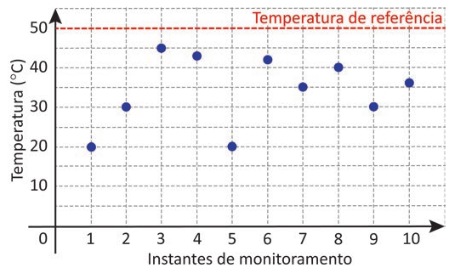
\includegraphics[width=0.4\textwidth]{q01img01.png}
                \end{figure}
            
            Quantas vezes, ao longo desse dia, o sistema de resfriamento foi acionado?

                \begin{enumerate}
                    \item 0
                    \item 1
                    \item 3
                    \item 4
                    \item 5
                    % gabarito: d
                \end{enumerate}

            \vest{ENEM} Uma fábrica de refrigerantes criou um novo tipo de bebida ao adicionar uma quantidade de um tipo de xarope a 10 litros de um refrigerante que já tem em sua fórmula 15\% desse xarope em sua composição. Com isso, 25\% da composição desse novo tipo de bebida é formada por esse xarope.
            
            Qual quantidade desse xarope, em litro, foi adicionada aos 10 litros de refrigerante para se criar esse novo tipo de bebida?

                \begin{enumerate}
                    \item $1$\vspace{8pt}
                    \item $\displaystyle\frac{4}{3}$\vspace{8pt}
                    \item $2$\vspace{8pt}
                    \item $\displaystyle\frac{5}{2}$\vspace{8pt}
                    \item $4$
                    % gabarito: b
                \end{enumerate}

            \columnbreak\vest{ENEM} Uma vacina foi testada em um grupo formado por 15 mulheres e 15 homens. Em testes clínicos realizados ao longo de vários anos, a vacina mostrou-se capaz de imunizar 80\% das mulheres e 60\% dos homens contra uma doença.  

            Um repórter, pretendendo fazer uma entrevista com uma das pessoas desse grupo, obteve uma listagem com os 30 números de telefone dessas pessoas, porém sem os respectivos nomes. Ele escolheu aleatoriamente um desses números e ligou para agendar a entrevista.  

            A probabilidade de que a pessoa para a qual o repórter telefonou seja um homem ou uma pessoa que tenha adquirido imunidade a essa doença com o uso da vacina é
                \begin{enumerate}
                    \item $\displaystyle\frac{1}{20}$\vspace{8pt}
                    \item $\displaystyle\frac{3}{10}$\vspace{8pt}
                    \item $\displaystyle\frac{7}{20}$\vspace{8pt}
                    \item $\displaystyle\frac{8}{10}$\vspace{8pt}
                    \item $\displaystyle\frac{9}{10}$\vspace{8pt}
                    % gabarito: e
                \end{enumerate}
            
            \columnbreak\vest{ENEM}Na produção de uma unidade de um produto, uma empresa gastava R\$ 40,00 na compra de matéria-prima e mais R\$ 40,00 em custos diversos. Essa empresa vendia esse produto por R\$ 120,00 a unidade.

            Em decorrência de mudanças no mercado consumidor, os custos diversos aumentaram em 50\%, embora o custo com matéria-prima tenha permanecido o mesmo. Assim, a empresa reajustará o preço de venda desse produto de forma que, ao conceder um desconto de 20\%, o lucro, em real, por unidade vendida permaneça o mesmo.

            De quanto será o reajuste, em real, no preço de venda desse produto?

                \begin{enumerate}
                    \item 16,00
                    \item 20,00
                    \item 25,00
                    \item 50,00
                    \item 55,00
                    % gabarito: e
                \end{enumerate}

            \vest{UERJ-2019} A partir do gráfico abaixo, o aumento da média anual de desempregados de 2014 para 2016 está mais próximo do seguinte percentual:

                \begin{figure}[H]
                    \centering
                    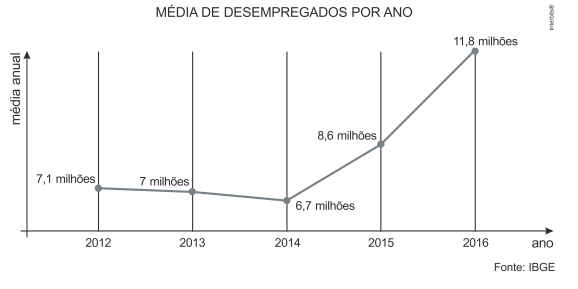
\includegraphics[width=0.4\textwidth]{q05im01.png}
                \end{figure}

                \begin{enumerate}
                    \item 68\%
                    \item 76\%
                    \item 80\%
                    \item 84\%
                    % gabarito: b
                \end{enumerate}

        \end{enumerate}
    \end{multicols*}
\end{document}